% Figure blocks for the article, one file per panel (requires \usepackage{subcaption} and \usepackage{graphicx}).
% Copy the PDFs of this folder to the Overleaf project. Labels are the same as in the manuscript.

% ---------------------------------------------------------------- Fig. 1 (flowchart)
\begin{figure}[!htbp]
\centering
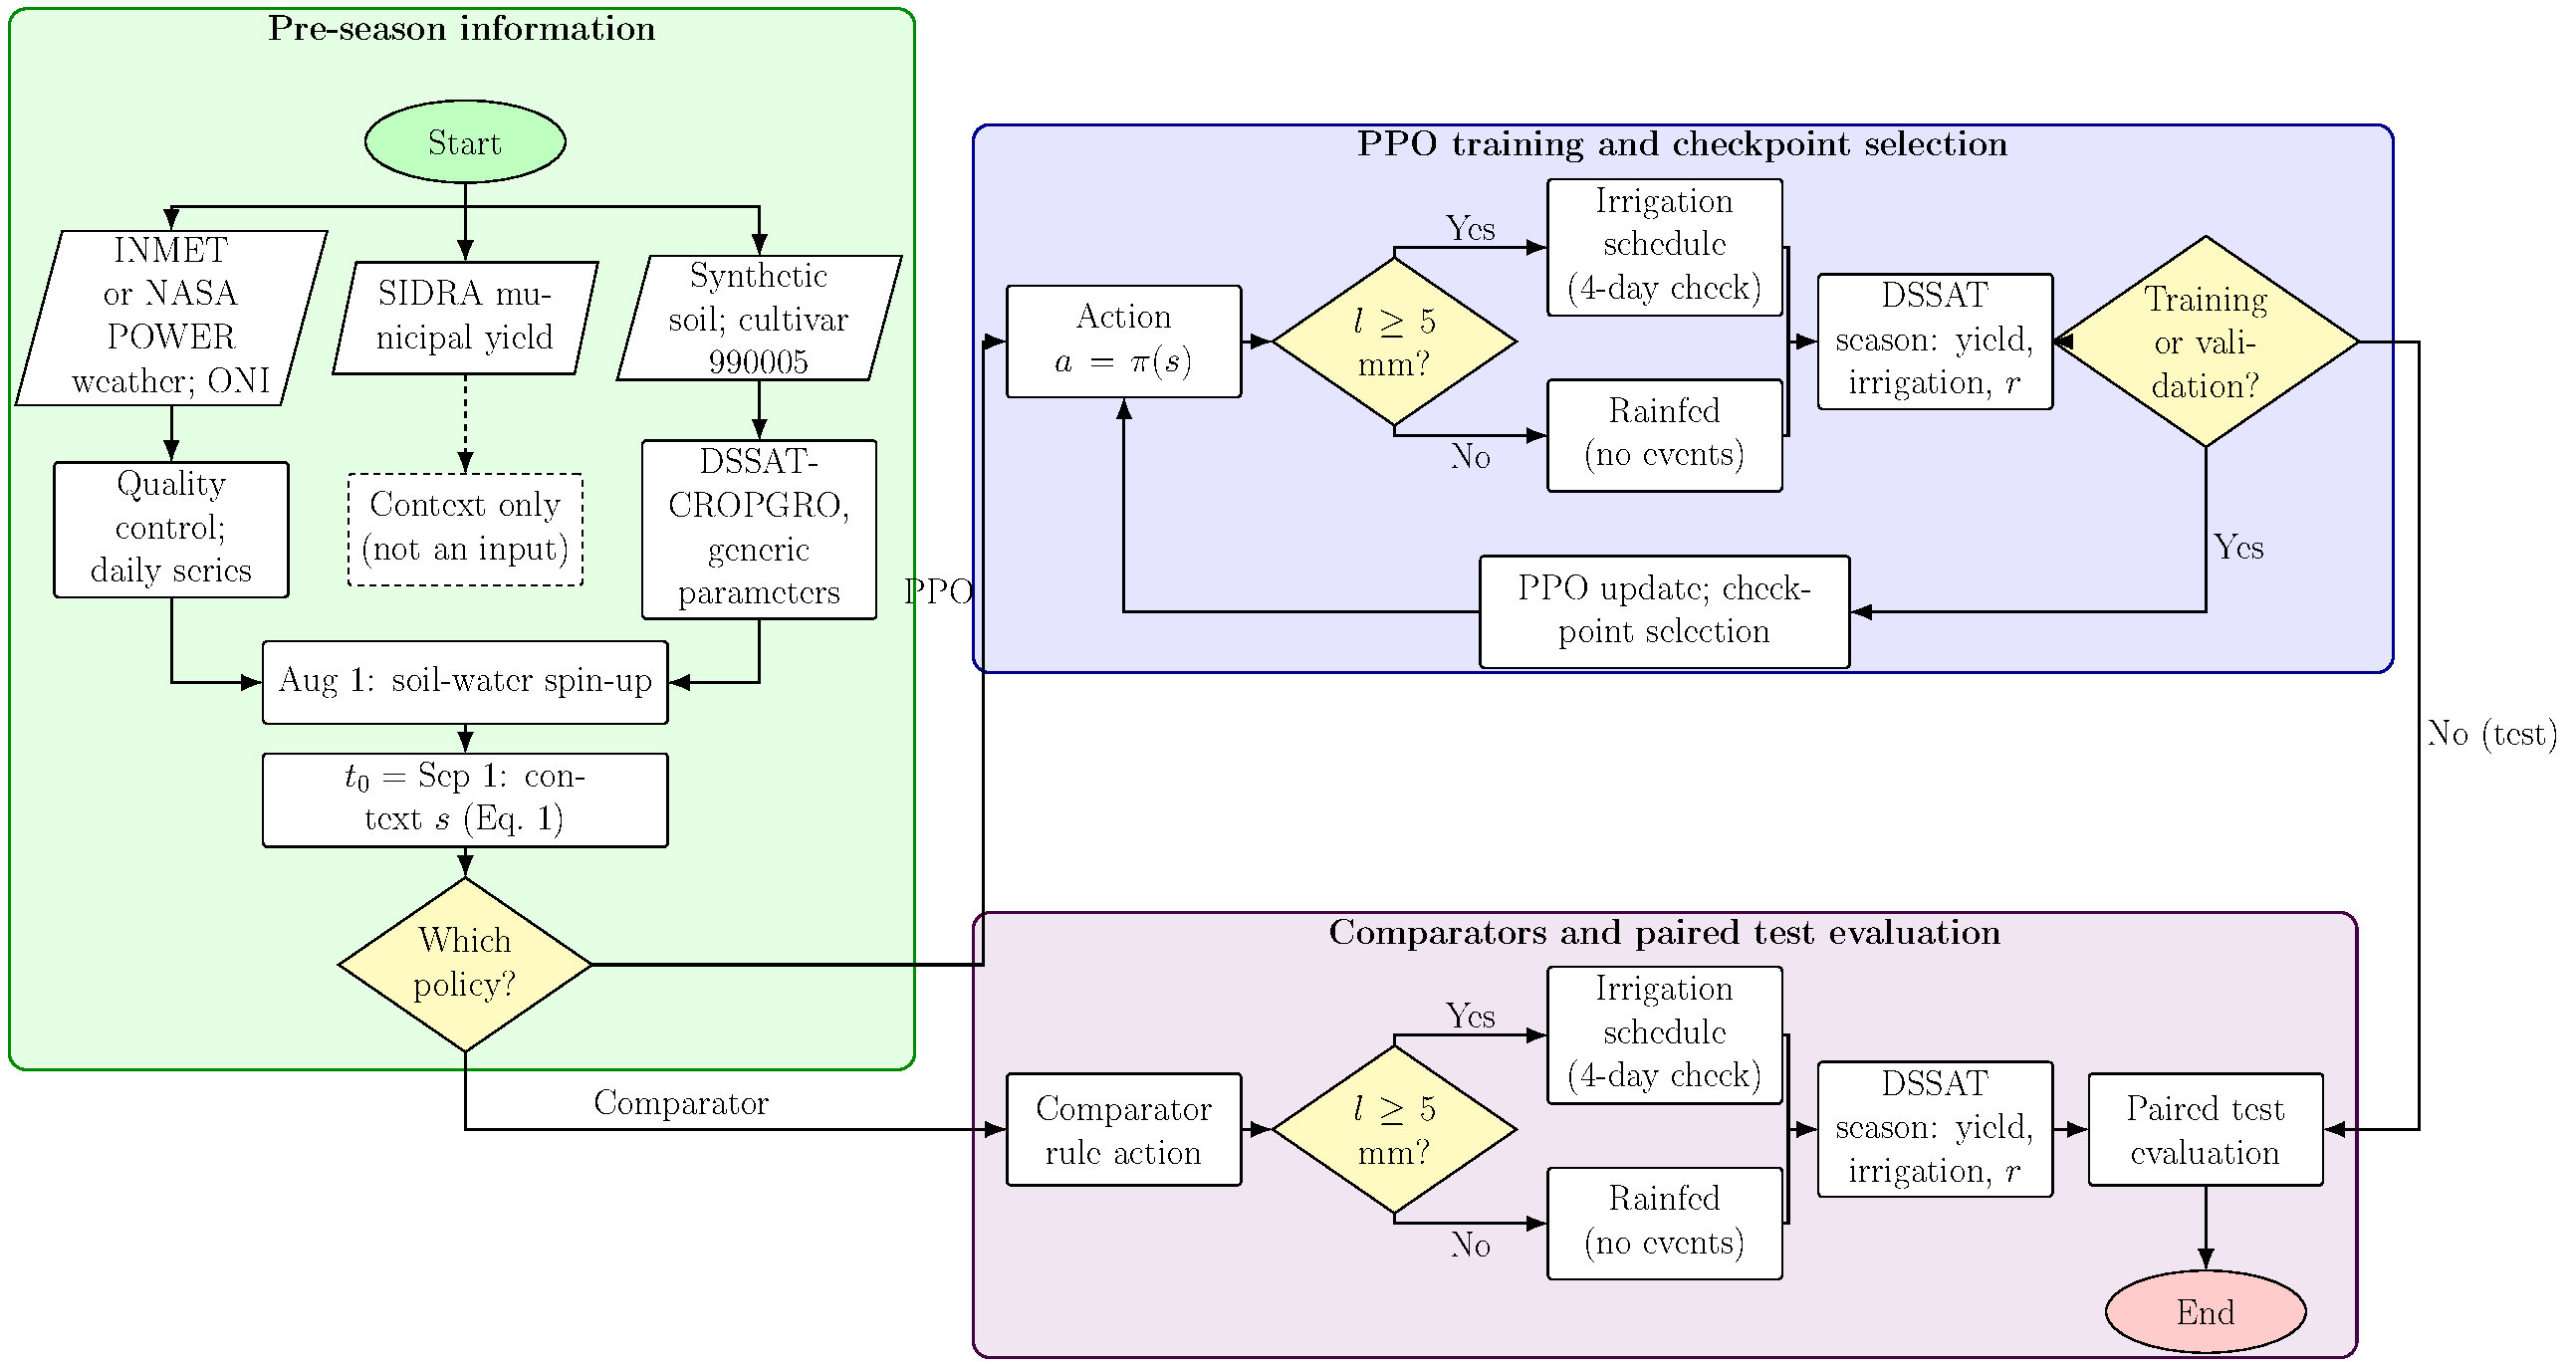
\includegraphics[width=\linewidth]{fig_flowchart_dssat_ppo.pdf}
\caption{System and decision timeline of the framework. Weather from the station (Experiment 1) or from NASA POWER (Experiment 2) passes through quality control to the context and to DSSAT; soil and cultivar use the generic DSSAT configuration; the SIDRA municipal series enters neither DSSAT nor the policy. The decision is taken on $t_0$ from the standardized pre-season context, the season is simulated after a soil-water spin-up from August 1, the irrigation rule is causal in time, PPO is updated on the training seasons and its checkpoint is selected on the validation seasons, and the paired evaluation uses seasons not used for development (Experiment 1: 2021--2024; Experiment 2: 2005--2024).}
\label{fig:flowchart_dssat_ppo}
\end{figure}

% ---------------------------------------------------------------- POWER vs INMET
\begin{figure}[!htbp]
\centering
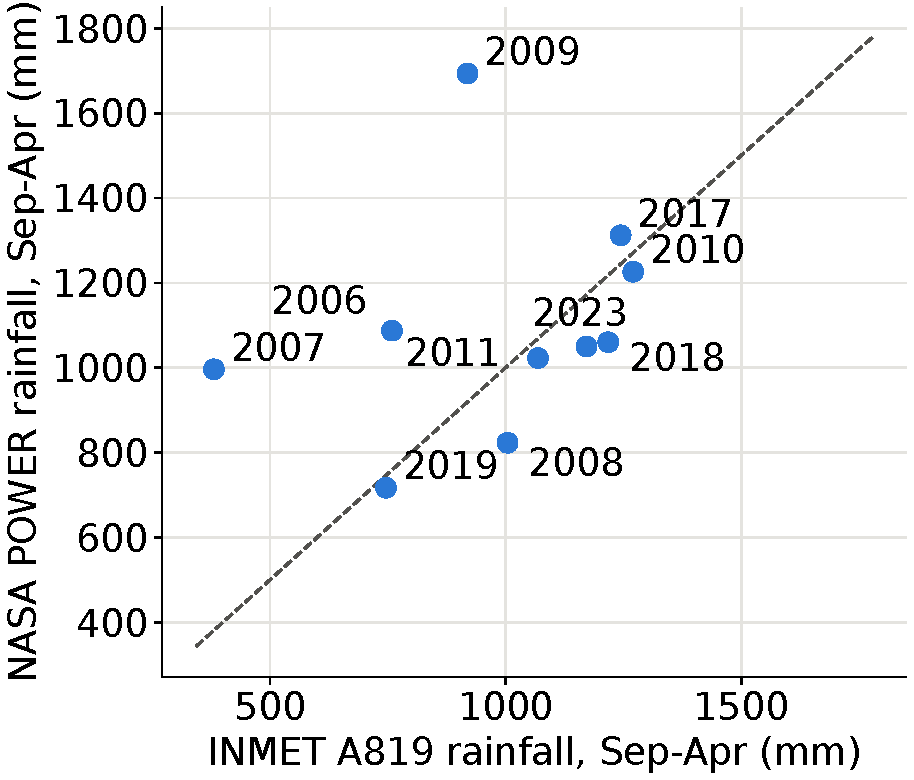
\includegraphics[width=0.5\linewidth]{fig_power_vs_inmet_season_rain.pdf}
\caption{September--April rainfall of the INMET A819 station and of NASA POWER for the seasons with at least 90\% valid station rainfall days. Dashed line: 1:1.}
\label{fig_power_inmet}
\end{figure}

% ---------------------------------------------------------------- Rainfed response
\begin{figure}[!htbp]
\centering
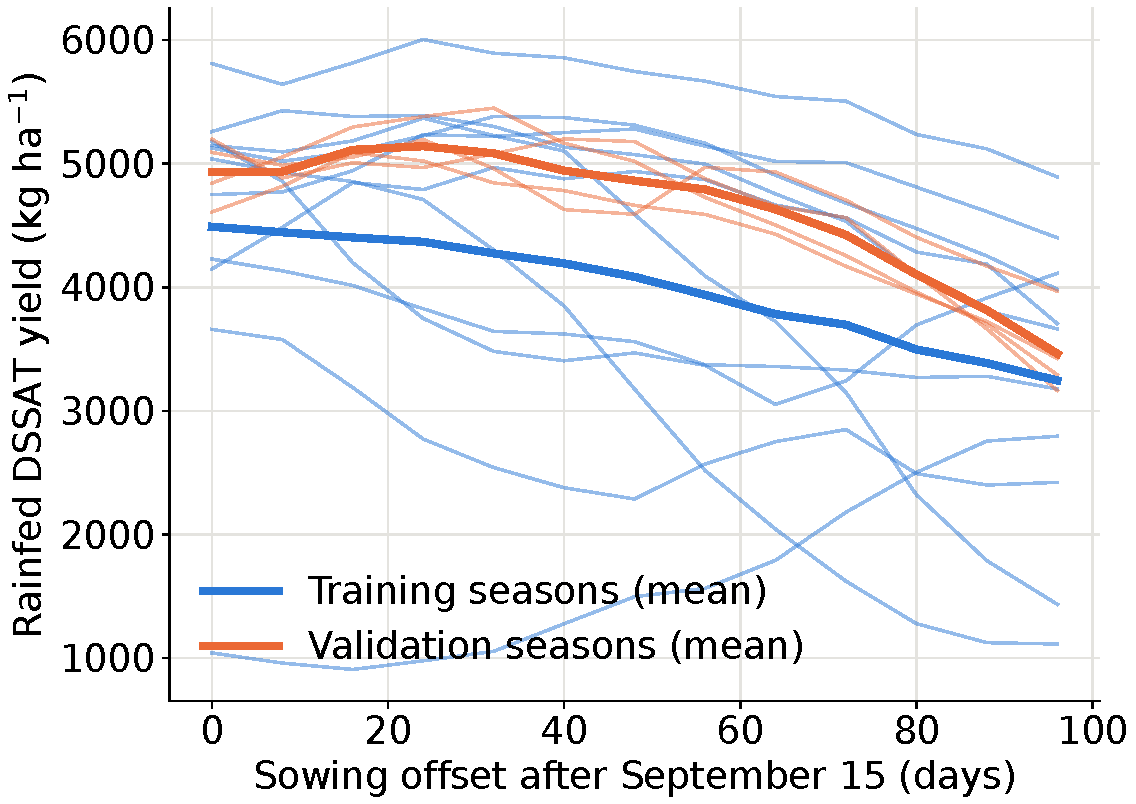
\includegraphics[width=0.6\linewidth]{fig_rainfed_sowing_response.pdf}
\caption{Rainfed DSSAT yield as a function of the sowing offset after September 15 in the INMET development seasons. Thin lines are seasons; thick lines are the means of the training (2006--2016) and validation (2017--2020) seasons.}
\label{fig_rainfed_response}
\end{figure}

% ---------------------------------------------------------------- Experiment 1 learning curves
\begin{figure}[!htbp]
\centering
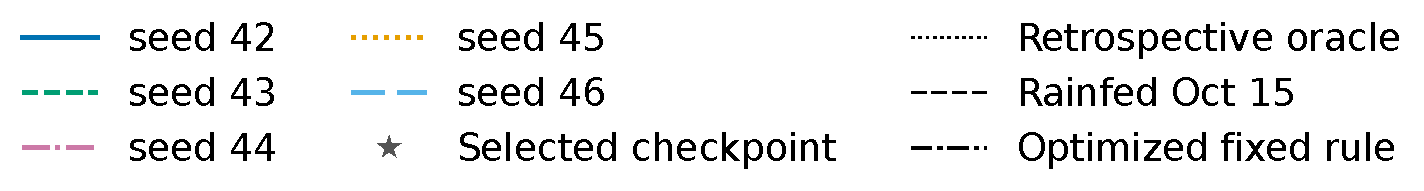
\includegraphics[width=0.95\linewidth]{fig_learning_curves_legend.pdf}\\[2pt]
\begin{subfigure}{0.48\linewidth}\centering
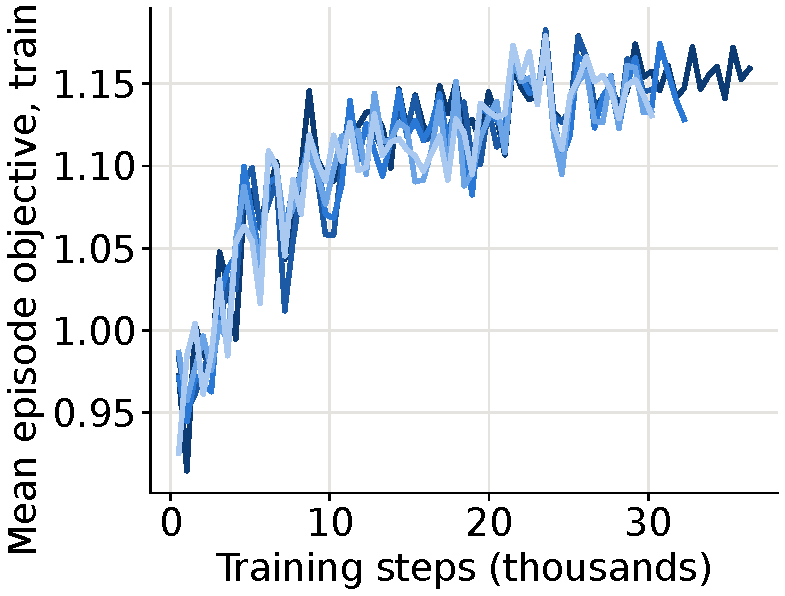
\includegraphics[width=\linewidth]{fig_learning_curves_a.pdf}
\caption{Training seasons 2006--2016}
\end{subfigure}\hfill
\begin{subfigure}{0.48\linewidth}\centering
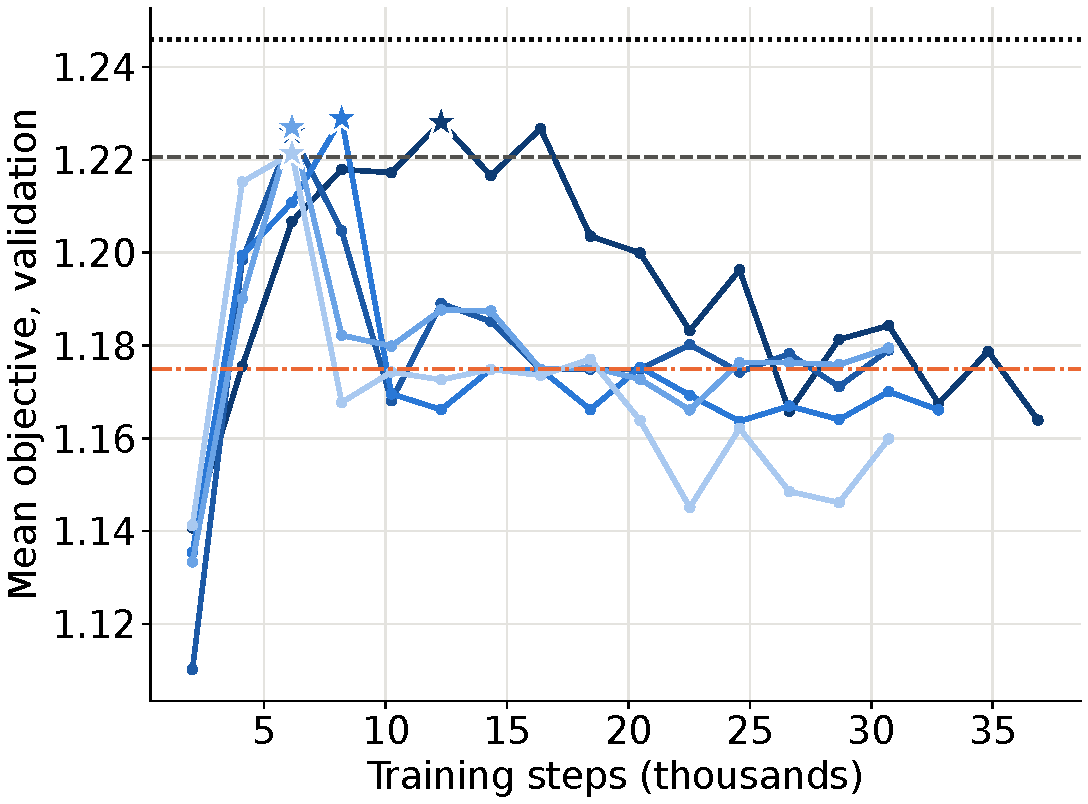
\includegraphics[width=\linewidth]{fig_learning_curves_b.pdf}
\caption{Validation seasons 2017--2020}
\end{subfigure}
\caption{Experiment 1: learning curves of PPO for seeds 42--46. (a) Mean objective of training episodes (stochastic actions, perturbed context) after each update of 512 episodes. (b) Objective of the deterministic policy on the four validation seasons, every 2,048 steps; stars mark the selected checkpoints. Horizontal lines: validation objective of the oracle, the rainfed October 15 schedule, and the fixed rule optimized on the training seasons.}
\label{fig_learning_curves}
\end{figure}

% ---------------------------------------------------------------- Experiment 1 PPO diagnostics
\begin{figure}[!htbp]
\centering
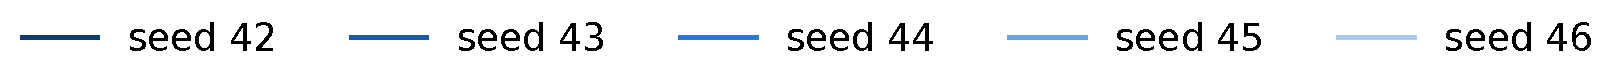
\includegraphics[width=0.8\linewidth]{fig_ppo_diagnostics_legend.pdf}\\[2pt]
\begin{subfigure}{0.48\linewidth}\centering
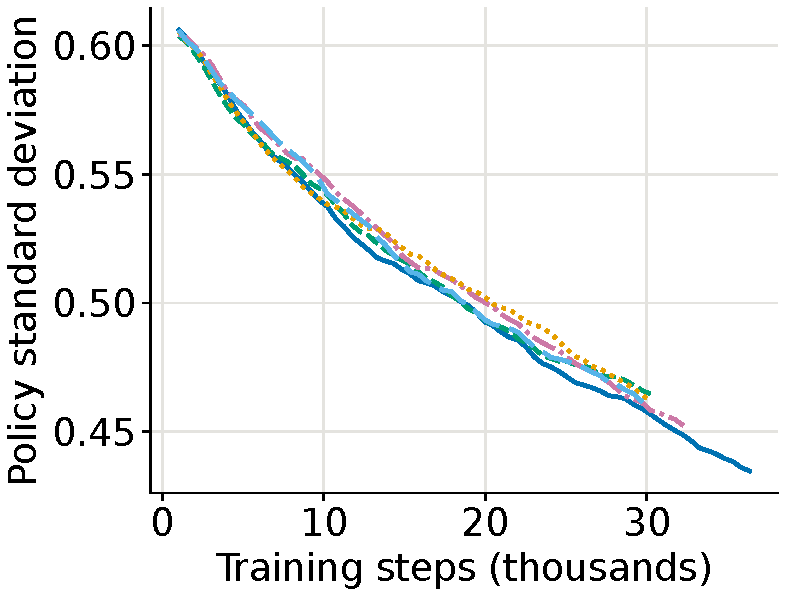
\includegraphics[width=\linewidth]{fig_ppo_diagnostics_a.pdf}
\caption{Policy standard deviation}
\end{subfigure}\hfill
\begin{subfigure}{0.48\linewidth}\centering
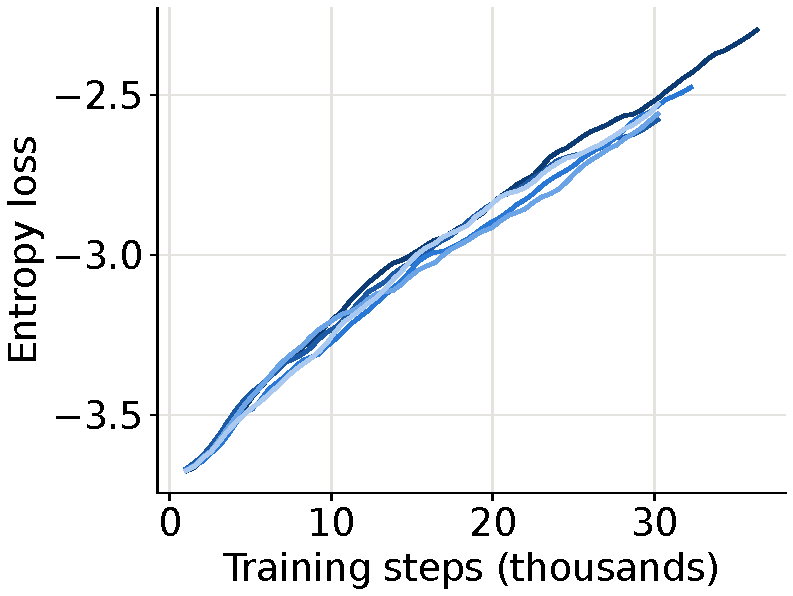
\includegraphics[width=\linewidth]{fig_ppo_diagnostics_b.pdf}
\caption{Entropy loss}
\end{subfigure}\\[4pt]
\begin{subfigure}{0.48\linewidth}\centering
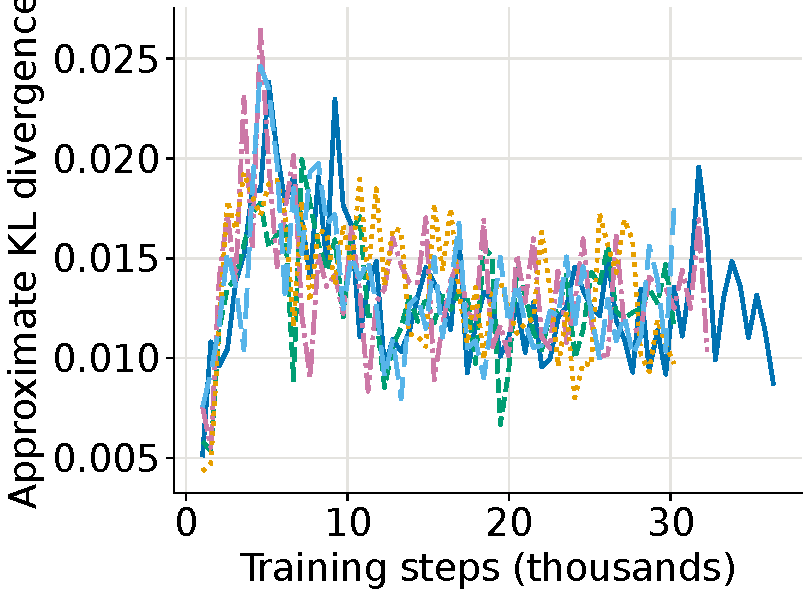
\includegraphics[width=\linewidth]{fig_ppo_diagnostics_c.pdf}
\caption{Approximate KL divergence}
\end{subfigure}\hfill
\begin{subfigure}{0.48\linewidth}\centering
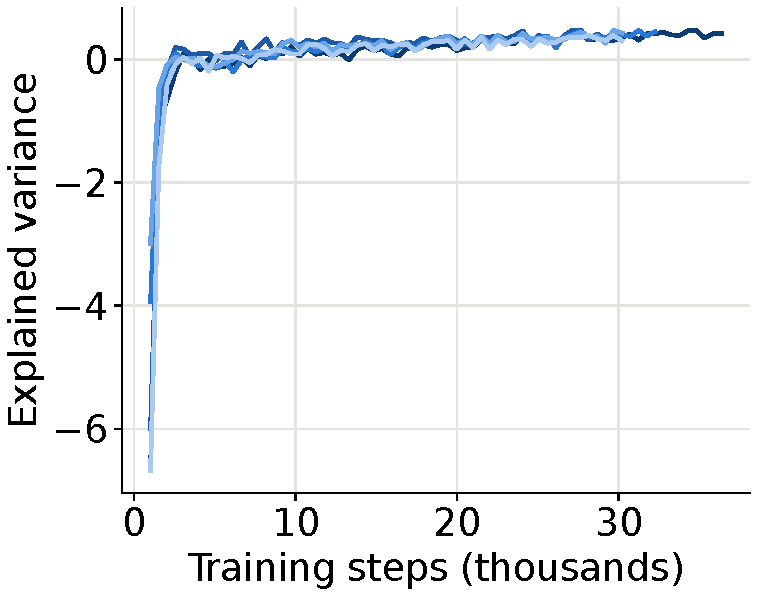
\includegraphics[width=\linewidth]{fig_ppo_diagnostics_d.pdf}
\caption{Explained variance of the value network}
\end{subfigure}
\caption{Experiment 1: PPO optimization diagnostics for seeds 42--46.}
\label{fig_ppo_diagnostics}
\end{figure}

% ---------------------------------------------------------------- Regularization
\begin{figure}[!htbp]
\centering
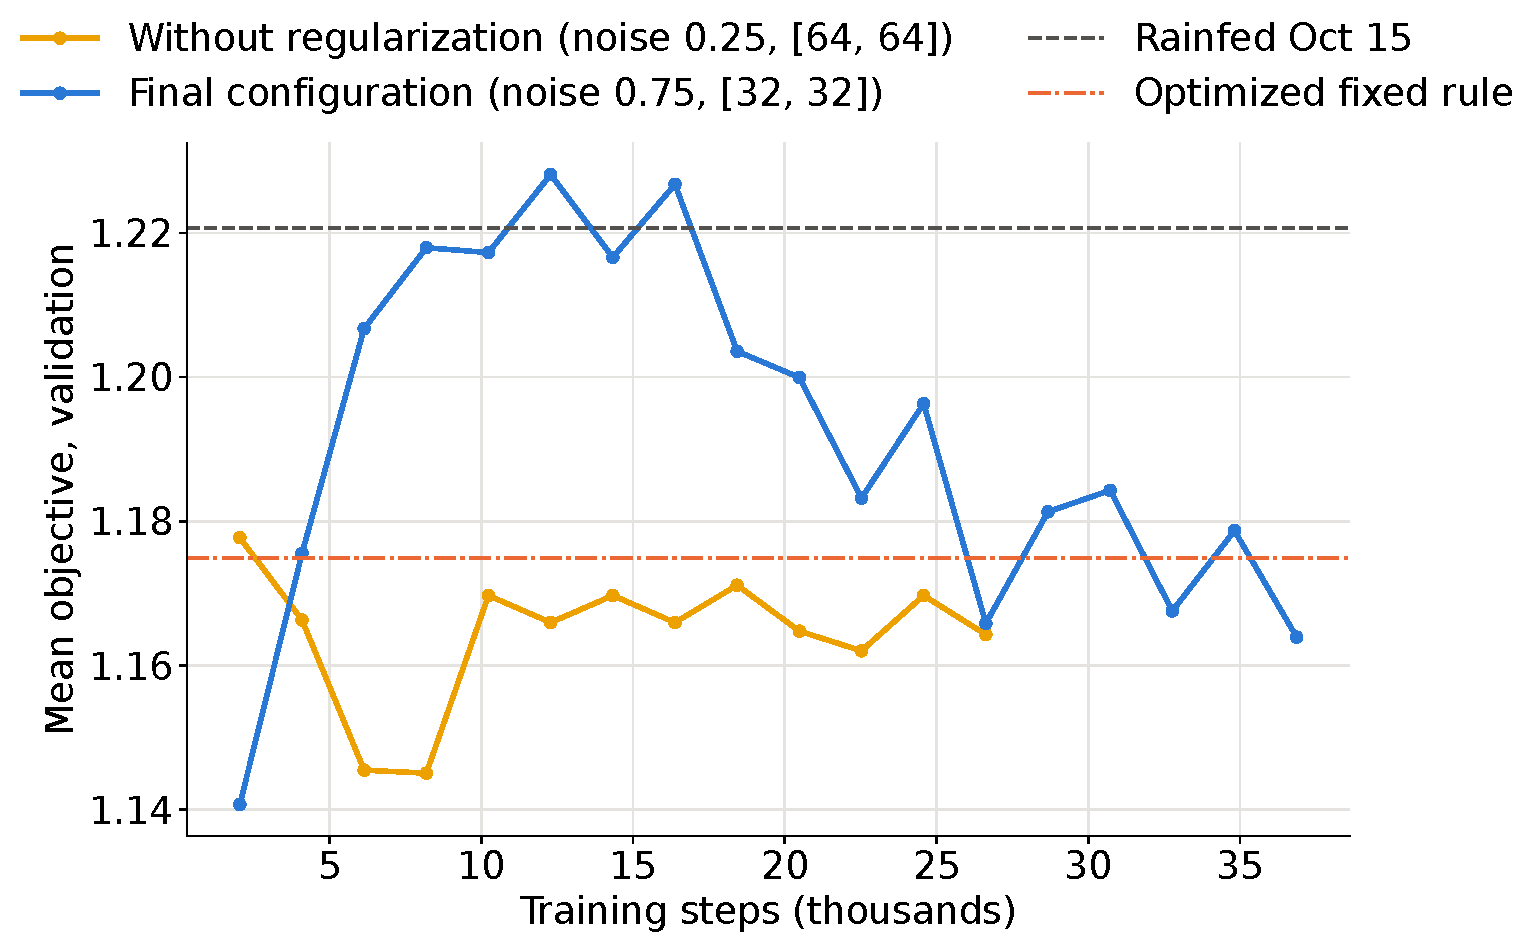
\includegraphics[width=0.7\linewidth]{fig_regularization_seed42.pdf}
\caption{Experiment 1: validation objective of seed 42 with the development configuration (context noise 0.25, two hidden layers of 64 units) and with the final configuration (context noise 0.75, two hidden layers of 32 units).}
\label{fig_regularization}
\end{figure}

% ---------------------------------------------------------------- Experiment 2 learning curves
\begin{figure}[!htbp]
\centering
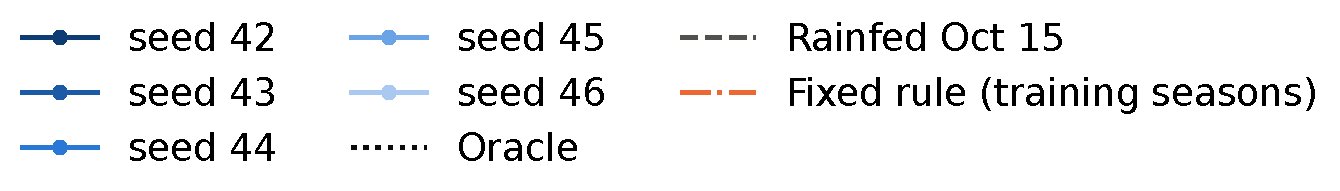
\includegraphics[width=0.95\linewidth]{fig_rolling_learning_curves_legend.pdf}\\[2pt]
\begin{subfigure}{0.32\linewidth}\centering
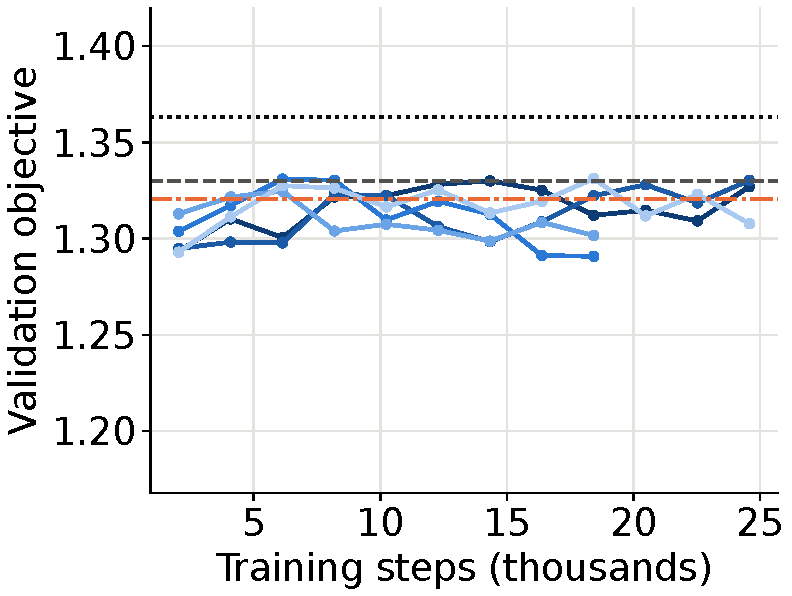
\includegraphics[width=\linewidth]{fig_rolling_learning_curves_a.pdf}
\caption{Test 2005--2008}
\end{subfigure}\hfill
\begin{subfigure}{0.32\linewidth}\centering
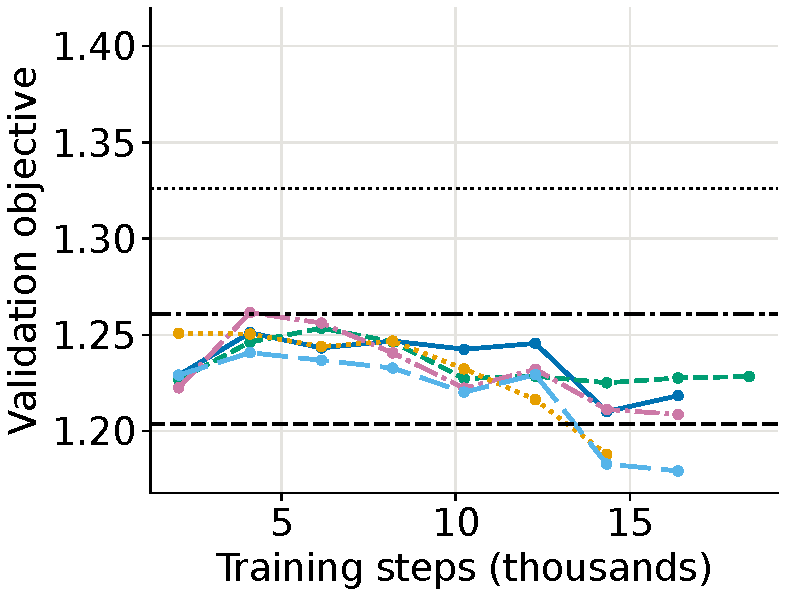
\includegraphics[width=\linewidth]{fig_rolling_learning_curves_b.pdf}
\caption{Test 2009--2012}
\end{subfigure}\hfill
\begin{subfigure}{0.32\linewidth}\centering
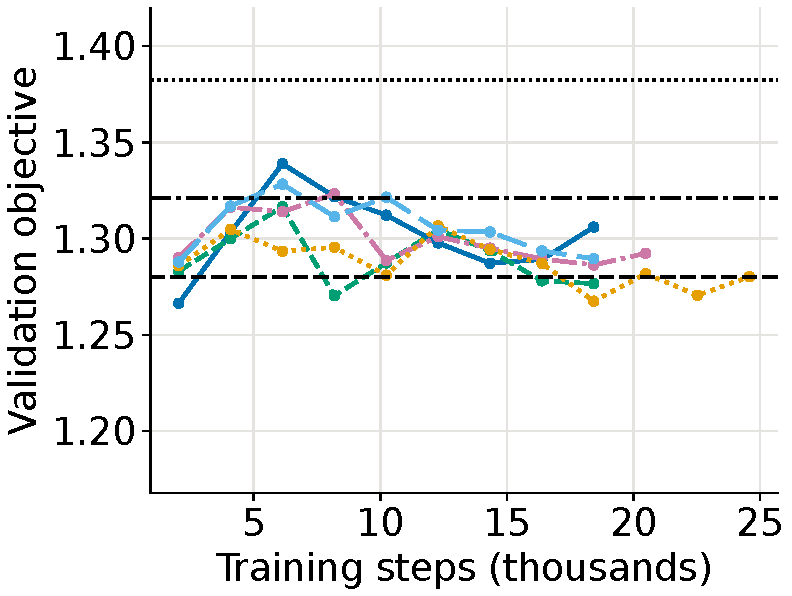
\includegraphics[width=\linewidth]{fig_rolling_learning_curves_c.pdf}
\caption{Test 2013--2016}
\end{subfigure}\\[4pt]
\begin{subfigure}{0.32\linewidth}\centering
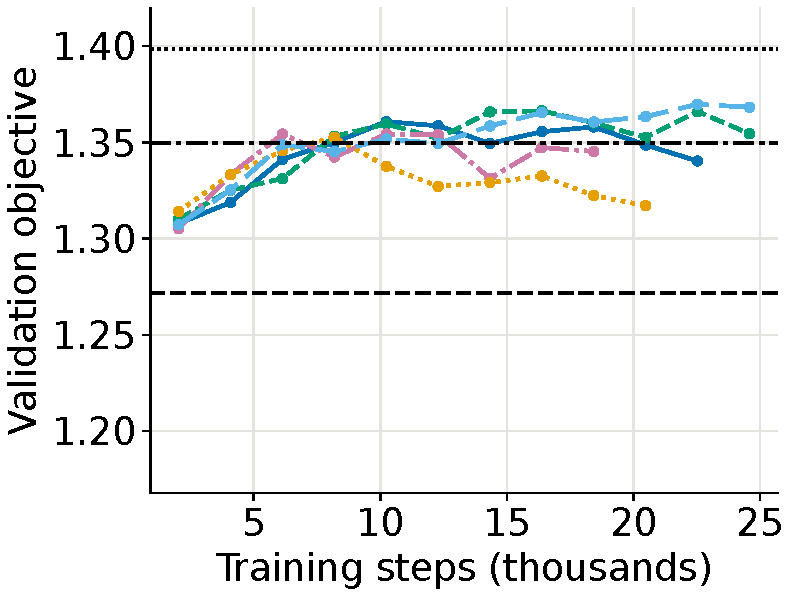
\includegraphics[width=\linewidth]{fig_rolling_learning_curves_d.pdf}
\caption{Test 2017--2020}
\end{subfigure}\hspace{0.02\linewidth}
\begin{subfigure}{0.32\linewidth}\centering
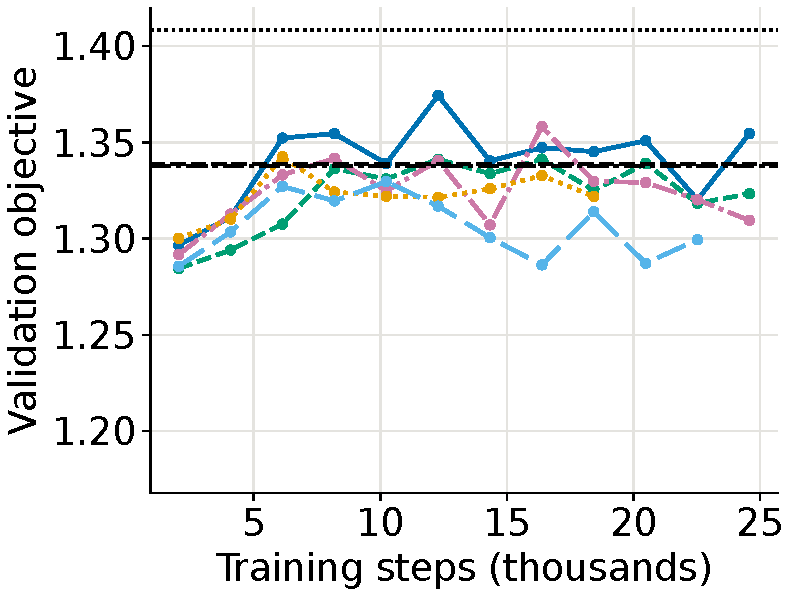
\includegraphics[width=\linewidth]{fig_rolling_learning_curves_e.pdf}
\caption{Test 2021--2024}
\end{subfigure}
\caption{Experiment 2: validation objective of the deterministic policy for each fold and seed, every 2,048 steps. The validation blocks are 2000--2004, 2004--2008, 2008--2012, 2012--2016 and 2016--2020. Horizontal lines: validation objective of the oracle, the rainfed October 15 schedule, and the fixed rule optimized on the training seasons of the fold.}
\label{fig_rolling_learning}
\end{figure}

% ---------------------------------------------------------------- Experiment 2 training diagnostics
\begin{figure}[!htbp]
\centering
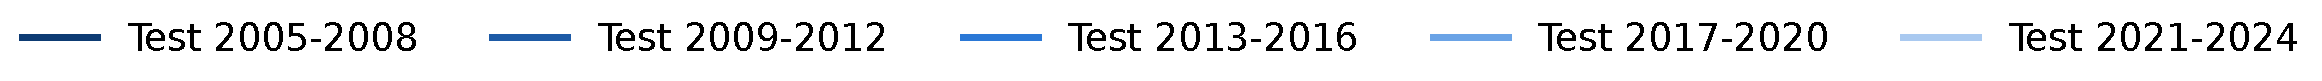
\includegraphics[width=0.95\linewidth]{fig_rolling_training_diagnostics_legend.pdf}\\[2pt]
\begin{subfigure}{0.48\linewidth}\centering
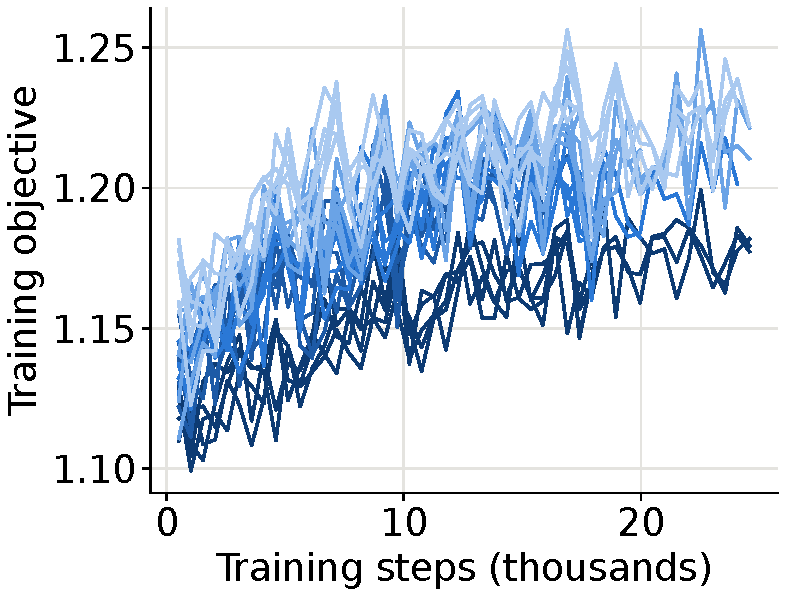
\includegraphics[width=\linewidth]{fig_rolling_training_diagnostics_a.pdf}
\caption{Mean objective of training episodes}
\end{subfigure}\hfill
\begin{subfigure}{0.48\linewidth}\centering
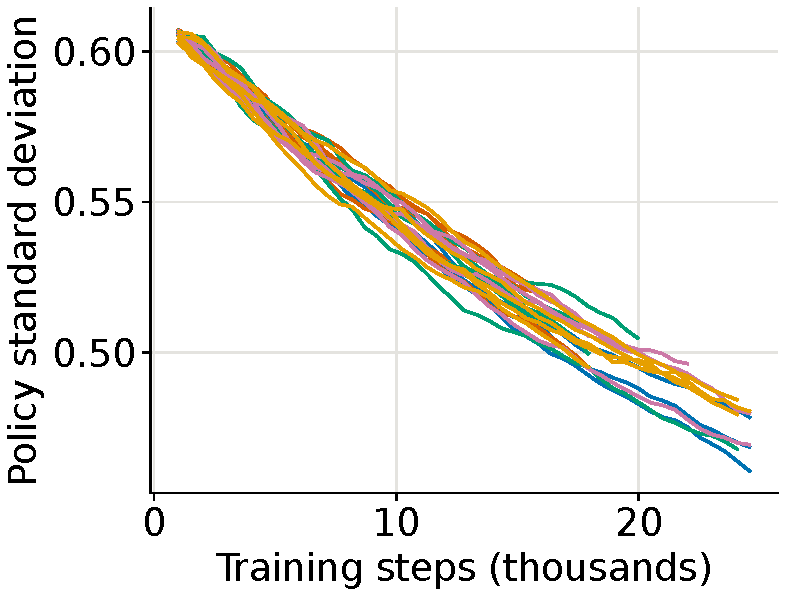
\includegraphics[width=\linewidth]{fig_rolling_training_diagnostics_b.pdf}
\caption{Policy standard deviation}
\end{subfigure}
\caption{Experiment 2: training diagnostics of the 25 runs, coloured by fold.}
\label{fig_rolling_diag}
\end{figure}

% ---------------------------------------------------------------- Paired yield
\begin{figure}[!htbp]
\centering
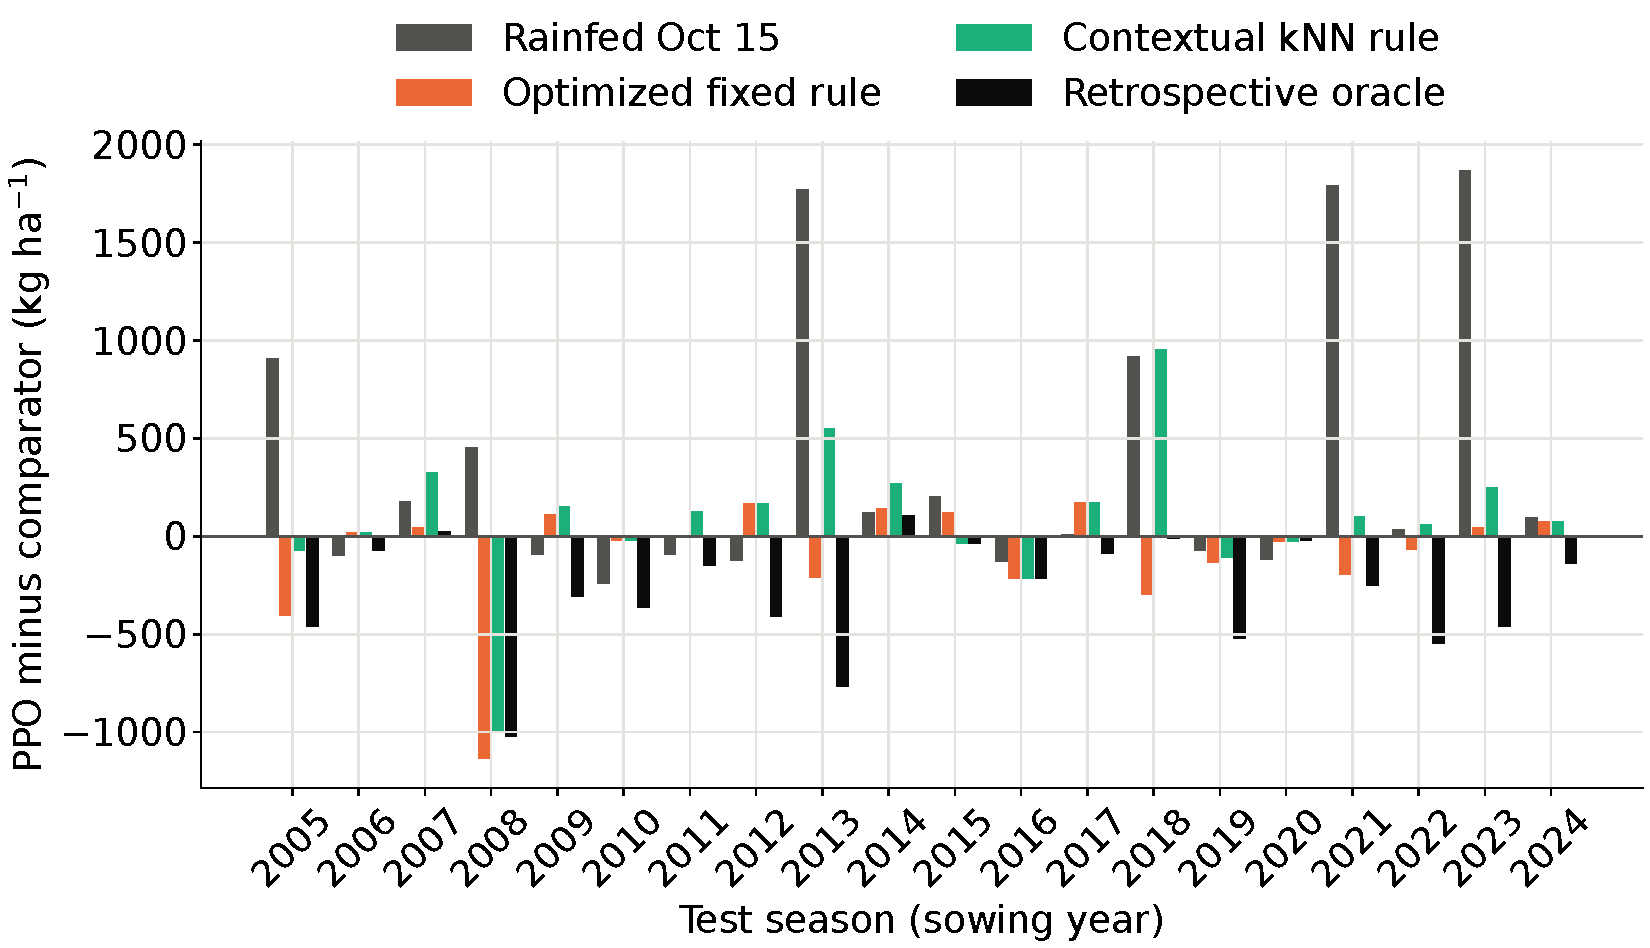
\includegraphics[width=\linewidth]{fig_rolling_paired_yield.pdf}
\caption{Experiment 2: paired yield differences between PPO (mean over seeds 42--46) and each comparator in the 20 test seasons.}
\label{fig_rolling_paired}
\end{figure}

% ---------------------------------------------------------------- Irrigation by season
\begin{figure}[!htbp]
\centering
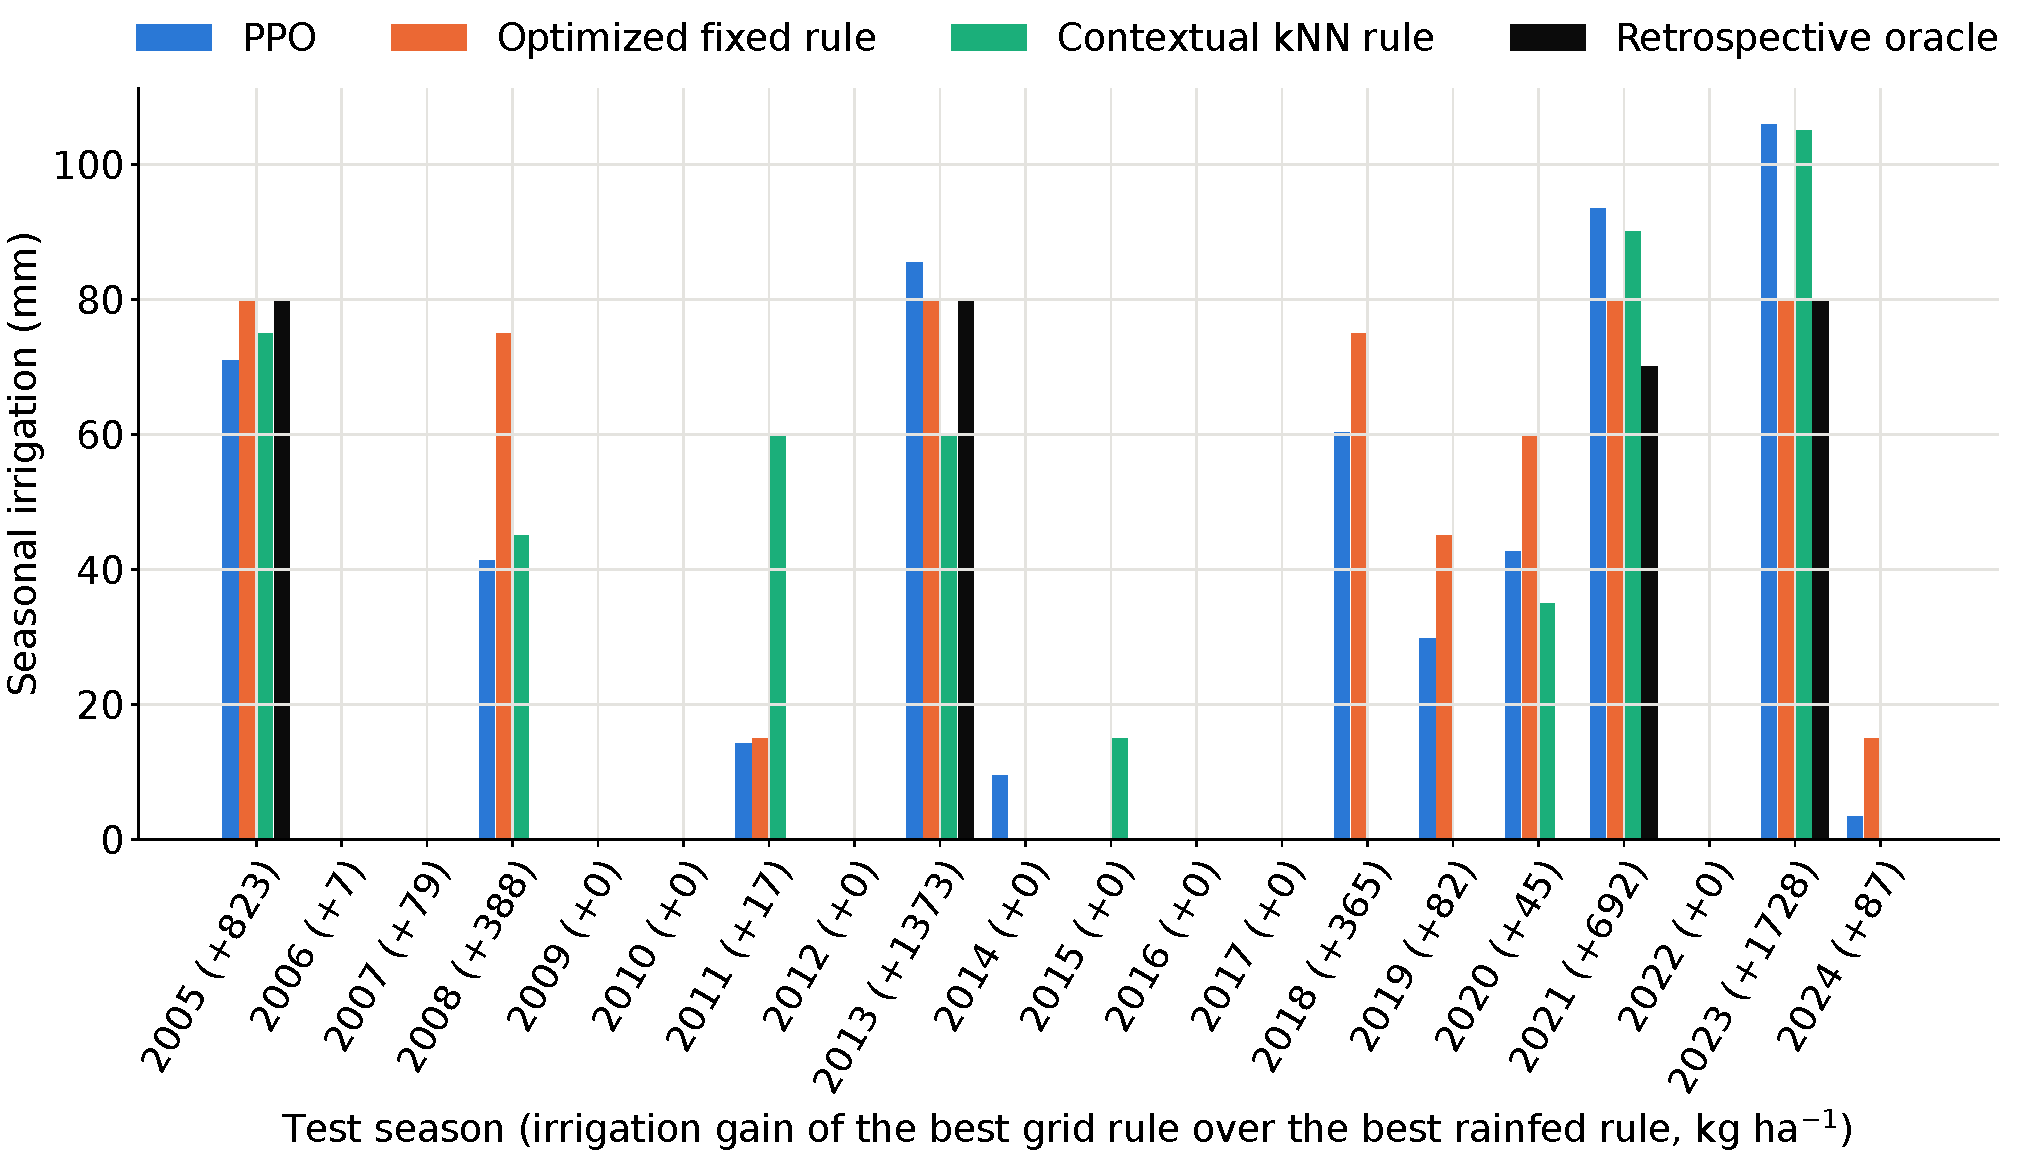
\includegraphics[width=\linewidth]{fig_rolling_irrigation_by_season.pdf}
\caption{Experiment 2: seasonal irrigation of PPO (mean over seeds 42--46), the optimized fixed rule, the $k$NN rule and the oracle in each test season. Values in parentheses: irrigation gain of the best grid rule over the best rainfed rule (kg ha$^{-1}$).}
\label{fig_rolling_irrigation}
\end{figure}

% ---------------------------------------------------------------- Context to action
\begin{figure}[!htbp]
\centering
\begin{subfigure}{0.32\linewidth}\centering
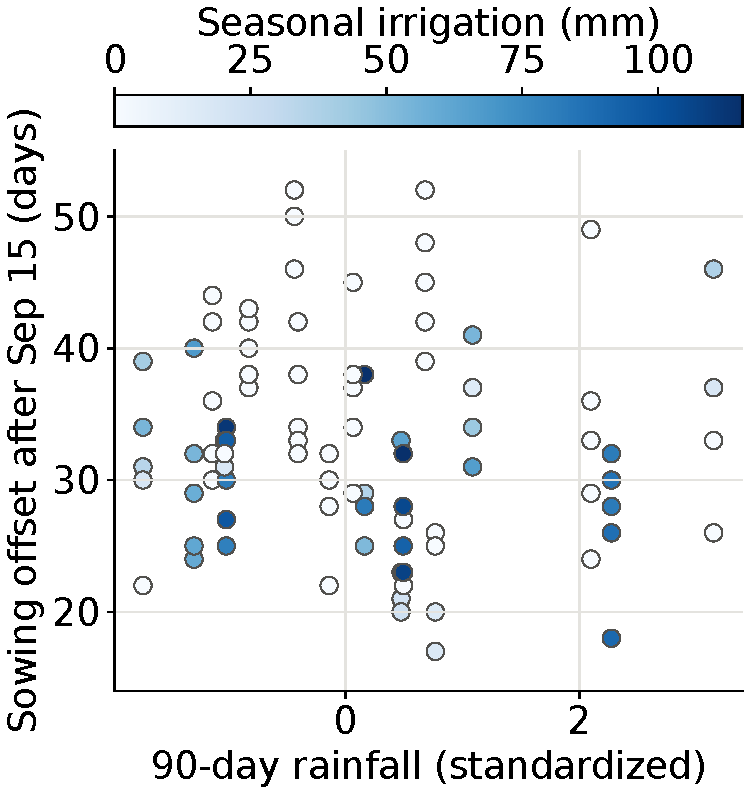
\includegraphics[width=\linewidth]{fig_rolling_context_action_a.pdf}
\caption{90-day rainfall}
\end{subfigure}\hfill
\begin{subfigure}{0.32\linewidth}\centering
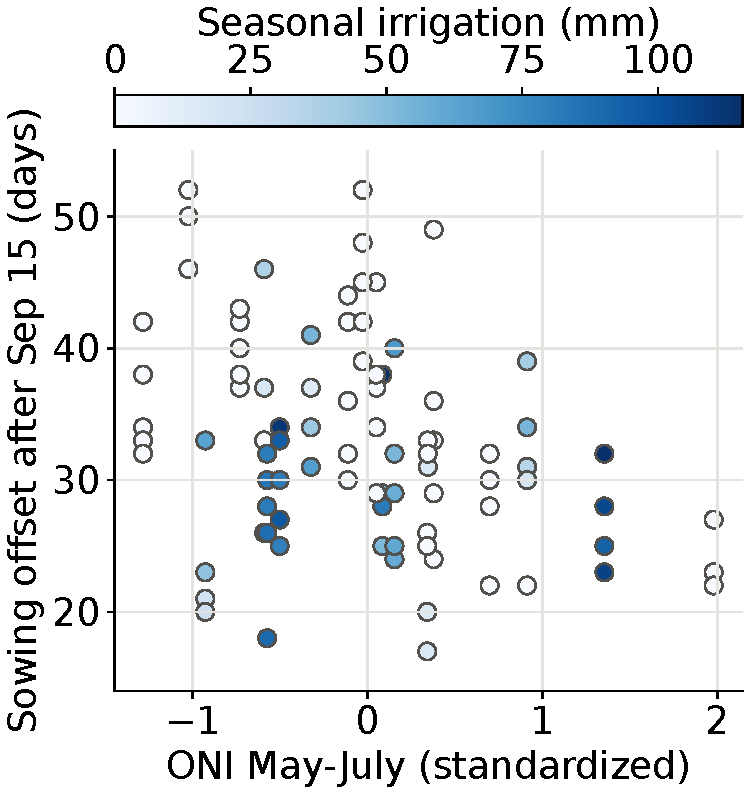
\includegraphics[width=\linewidth]{fig_rolling_context_action_b.pdf}
\caption{ONI May--July}
\end{subfigure}\hfill
\begin{subfigure}{0.32\linewidth}\centering
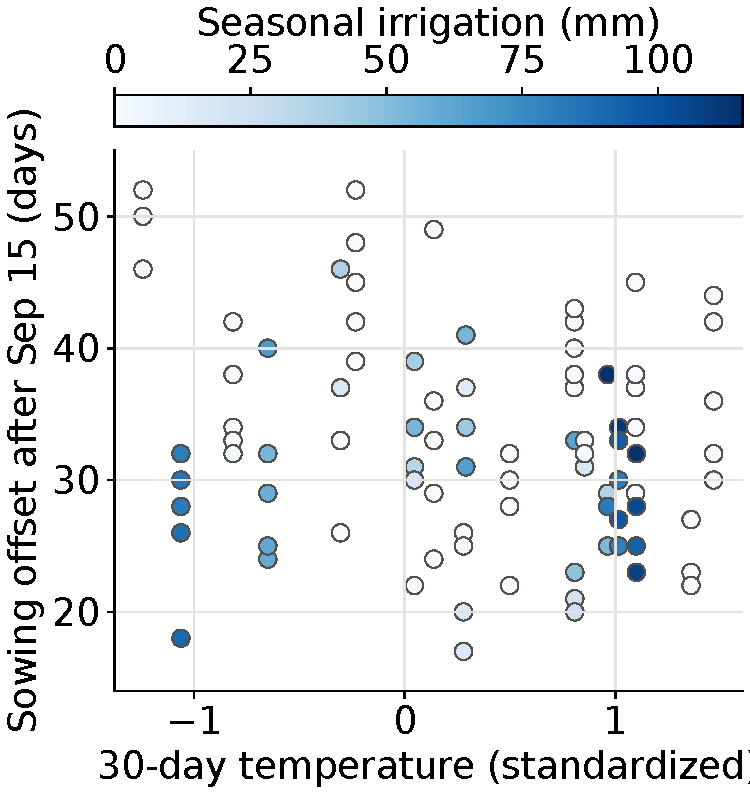
\includegraphics[width=\linewidth]{fig_rolling_context_action_c.pdf}
\caption{30-day temperature}
\end{subfigure}
\caption{Experiment 2: sowing offset selected by PPO against three standardized context variables of the test seasons (one point per season and seed); colour: seasonal irrigation.}
\label{fig_context_action}
\end{figure}

% ---------------------------------------------------------------- Water frontier
\begin{figure}[!htbp]
\centering
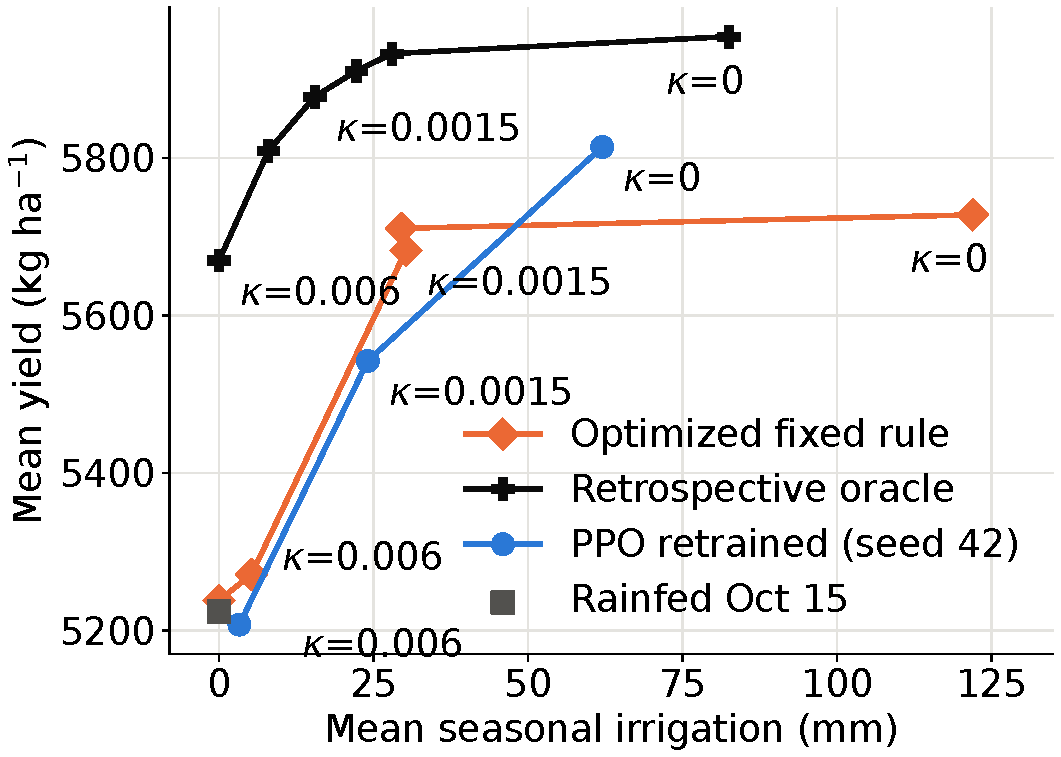
\includegraphics[width=0.7\linewidth]{fig_rolling_water_frontier.pdf}
\caption{Experiment 2: mean yield and mean seasonal irrigation over the 20 test seasons for the optimized fixed rule and the oracle re-selected at six water penalties ($\kappa$ from 0 to 0.006 mm$^{-1}$; labels on the three penalties used for PPO), PPO with seed 42 at three penalties, and the rainfed October 15 schedule.}
\label{fig_rolling_frontier}
\end{figure}
